\documentclass[12pt]{book}
\usepackage{mathtools}
\usepackage{graphicx}
\usepackage[utf8]{inputenc}
\usepackage{float}
\usepackage{tabularx}
\usepackage{chngpage}
\usepackage{amsthm}
\usepackage{mathtools}
\usepackage{amsfonts}
\usepackage{tikz}
\usepackage{amssymb}
\usepackage{gensymb}
\usepackage{wrapfig}
\usepackage{enumerate}
\usepackage{braket}
\usepackage{pgfplots}
\usepackage{bbm}
\usepackage{fancyhdr}
\usepackage{emptypage}


%\numberwithin{equation}{section}
\newcommand{\R}{\mathbb{R}}
\newcommand{\F}{\mathcal{F}}
\renewcommand{\L}{\mathcal{L}}
\newcommand{\C}{\mathbb{C}}
\renewcommand{\H}{\mathcal{H}}
\newcommand{\Sum}{\sum_{n=0}^\infty}
\newcommand{\Res}[1]{\text{Res}f(z)\Big|_{#1}}
\newcommand{\vettore}[1]{\overrightarrow{#1}}
\newcommand{\p}{\mathbf{p}}
\newcommand{\x}{\mathbf{x}}
\renewcommand{\r}{\mathbf{r}}


\usepackage[a4paper, inner=1.5cm, outer=3cm, top=3cm, 
bottom=3cm, bindingoffset=1cm,headheight=110pt]{geometry} 


\pagestyle{fancy}
\fancyhf{}
\fancyhead[LE]{\leftmark}
\fancyhead[RO]{\rightmark}
\fancyfoot[C]{\thepage}
\begin{document}
\begin{titlepage}
  \pagestyle{empty}

  \begin{center}
    {\bfseries
      \Large {\huge U}NIVERSITY OF {\huge T}RENTO}

    \vspace{0.2cm}

    {\Large Department of Physics}

    \vspace{0.5cm}

    \begin{center}
      
\includegraphics[width=0.3\textwidth]{img/logo_unitn.png}
    \end{center}

    \vspace{0.5cm}

    {\bfseries \Large Degree course in Physics}

    \vspace{0.3cm}
    \line(1,0){338}
    \vspace{0.3cm}

    {\Large Final Thesis}

    \vspace{2.5cm}

    {\huge \textsc{Generation and manipulation of}}

    \vspace{0.4cm}

    {\huge \textsc{entangled photon pairs in}}

     \vspace{0.4cm}

     {\huge \textsc{coupled resonators}}
    

    \vspace{3.0cm}


    \large
    \begin{center}
      \begin{tabular}{ccc}
        {\bfseries Supervisor} &
        \hspace{5cm}
        {\bfseries Candidate} \\

        Prof. Lorenzo Pavesi &
        \hspace{5cm} Marco Canteri \\


      \end{tabular}
    \end{center}
    \vspace{2cm}

    {\bfseries \large Academic year 2016-2017}
    \vfill
  \end{center}
\end{titlepage}

\tableofcontents
\chapter{Introduction}
The aim of this thesis is to describe a theoretical model for the generation of entangled photons inside silicon optic chips. In particular, the structure i'm going to study is composed by two microrings side coupled to two channel waveguide. The geration of entangled photons is obtained exploiting non linear proprieties of silicon. In order to fullfil this goal, the second chapter gives a description of the needed basic structures, the microrings and the waveguides and how we can describe their behaviour using a mathematical formalism. The third chapter is devoted to the explanation of the physics behind the phenomena and the mathematics which can be used to carry out the calculation. Finally in the fourth chapter the model and the results are presented. The rest of the introduction is an overview on photonics. 
\section{Integrated optics}
The microelectronic has been widely succesfull and it was a revolution that has changed our daily life and works, nowdays microelectronics is present almost everywhere. The great success of this technologies is due to many reasons, one of them is the computational power of a small chip which for the Moore's law is predicted to be doubled every to years. The prediction still holds today, but we are reaching saturation point, in fact the improvements were possible by increasing the clock frequencies of the processing units, this kind of improvement faces several problems, such as heating power, antenna effects and RC time delays. Therefore, in order to keep the improvements going, the approch used is now to increase the number of processing units, but the problems are still present, they are only changed. The cores needs to communivate among them, so the problem is to realize efficient communication with high bandwidth and low power consumption. Photonics is a platform that can be used to achive such goal, with light is possible to realize ultra-high speed switch, it has low power consumption and it doesn't have electromagnetic noise. Several platform has been developed with different media, for example silicon, lithium niobate, arsenium gallium compounds. Since the electronics industry is based on silicon, Silicon-on-Insulator (SOI) photonics is a promising platform to build optical chip. The technologies used for the fabrication of silicon chip is well studied and understood, it reached a high maturation and the industry and the infrastructure already exist. Futhermore silicon photonics has the compatiblity with the CMOS technlogy used is electronic chip, hence hybrid chip with electronics and photonics can be realised. Another important feature of silicon is the transparency at the important Telecom wavelenghts 1300-1600 nm, which allows the fabrications of photonic circuit with very low power loss. The aim of silicon photonics is to follow the philosophy behind microelectronics, small chip composed by few building block that can be used to build different devices changing the topology if the chip, and to realize this building block with fewer materials as possible and with a standard among the manifacturies.\\
In quantum mechanics light has been quantized and the single particle, photon, has quantum proprietis.\\
A silicon optic chip is realised with three different layers as depicted in figure \eqref{SOIstructure}, at the bottom we can find the substrate, a silicon layer which provides a base and a stable structure for the chip, just above it there is a layer made of silicon dioxide called cladding and finally at the top there is another silicon layer called core. The thickness of the substrate and the cladding is in the order of some $\mu m$, while the core has an height in the order of few hundreds $nm$. The refractive index of silicon is $n_{Si} \simeq 3.5$ in the range of the Telecom wavelenghts, while the refractive index of silicon dioxide is $n_{SiO_2}\simeq 1.54$ in the same range, this allows the confinement of light in the core layer by total internal refraction. Exactly like in optical fiber the light travelling in the core layer when reaches the boundaries with the layer underneath or with the air (refractive index $\simeq 1$) is reflected back if the angle of incidence is greater then a critical angle. 
\begin{figure}
\centering
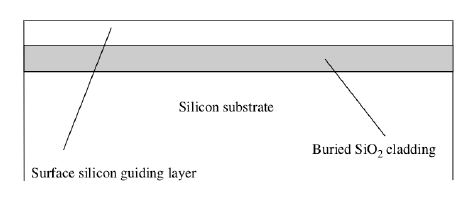
\includegraphics[width = .7\textwidth]{img/SOIstructure}
\caption{SOI chip layer structure}
\label{SOIstructure}
\end{figure}
\section{Waveguides}
The most important block for a optical chip is a waveguide. The signal is carried inside this block by confinement of light inside of it. The confinement is due to total internal reflection. Consider the system in figure [], when the light strikes the medium boundary, a part of it get reflected, while another part is transmitted. If the angle of incident is less then a critical angle $\theta_c$, the light is completly reflected. Indeed, the angle of the refracted light is given by the snell's law
\[n_1 \sin \theta_1 = n_2 \sin \theta_2\]
which can be written as
\[\sin \theta_1 = \frac{n_1}{n_2}\sin \theta_2\]
if we impose $\theta_2$ to be at least $90\degree$, we obtain
\[\sin \theta_1 = \frac{n_1}{n_2} \implies \theta_1 = \arcsin\left(\frac{n_1}{n_2}\right) \]
this is the critical angle, it's clear from the equation that the critical angles exist only if $n_1/n_2<1$, i.e $n_1>n_2$. Hence the phenomenon of total internal reflaction occurs only when light is inside a medium with a refractive index greater than the surroundig's one. This is the case of SOI device, where the light propagates inside a layer of silicon shandwiched by a layer of silica and the air which have a refractive index smaller than the silicon's.\\
Inside a waveguide, several modes of propagation are possible, the electric field profile $E_m$ follows the Helmoltz equation:
\[(\nabla_{xy}^2 + \beta_m)E_m(x,y)= \frac{\omega^2}{c^2}n^2E_m(x,y)\]
where $\beta_m$ is called the modal propagation costant, and it's given by $\beta_m = \frac{\omega}{c}n_{eff}$ where $n_{eff}$ th effective index. $m$ is an integer quantity that represent the discrete mode of propagation.


An important physical conseguence can be deduced from this equation, the electric and the magnetic field cannot be discontinuos at a boundary, so the field is not totally inside the waveguide. but a small part can be found also outside. Indeed Maxwell's equations impose boundary conditions on the electric and magnetic field. The solution of those equations outside the waveguide must be vanishing and it cannot transport energy, otherwise the light would not be confined inside the waveguide, the only solution is to have a exponentially decreasing wave, such wave is called the evanescent wave. This evanescent wave explain why there is the effective index in the formula of the modal propagation costant, the wave, which travels inside the waveguide, propagates inside a medium with fixed refractive index and its tail propagates outside the waveguide, so it has a different refractive index, therefore the effective index accounts for this phenomenum.
Evanescent field are also important when two waveguides are really close to each other, if light travel inside a waveguides and its evanescent tail reach the second waveguide there is transfer of energy and the light can penetrate into the core of the neighboring one. This allows the coupling of different waveguides or, as we'll see later, the coupling between a waveguide and a resonator. It's also interesting to look at the quantum description of this effetc, a photon is described by a wave function which is a solution of the Schroedinger equation, in the same mathematical way of the maxwell's equations, this impose the continuity of the wavefunction across the medium bondary. If two waveguides are close, the wave function is non zero insideboth waveguides, so a photon have a non zero probability to pass through the gap and change waveguide, in quantum mechanics this effect is called quantum tunneling. 
\section{Resonator}
A waveguide can be bended and closed to itself to provide coherent feedback to the circulating light. Such devides is called a resonator and it can have different shape, such as ring, racetracks, disk, toroids. Due to the size of these device they are called microresonator. For the ease of the calculation we'll treat only microrings with fixed radius, typically this radius is in the order of the $\mu m $. Inside a ring resonator light interferes constructively if it's satisfied $n_{eff} L = m \lambda_m$, where L is the lenght of the circunference, m an integer and $\lambda_m$ is the light wavelenght. A consequence of constructive interference is that inside the resonator a large amount of energy is stored and the intesity of the field is enanched. A strong electric field can cause non linear effects, this is a reason on the importance of resonator, with low power input it's possible to have non linear effects that usually require a source with more power because they are very small. \\
There are mainly two ways to create circut with the two basic block just described, the first one is a waveguide side coupled to a single ring, this configuration is called All Pass Filter (APF), while if there are two waveguide coupled to a single ring, the configuration is called Add-Drop Filter (ADF). In figure [] we can see both configuration. The coupling is possible by means of the evanescent wave, since the gap between the waveguide and the ring is really narrow (order of $\simeq 100\, nm$).\\
Coupling can be seen as a quad port beam splitter and the relationship between the complex amplitudes of waves in input and output can be represented with the following matrix
\[M = \begin{pmatrix}
r & ik \\
ik & r\\
\end{pmatrix}\]
where $r$ is the reflection coefficient and $k$ is the coupling coefficient, they satisfy $r^2 +k^2 = 1$. The elements of the matrix can be found imposing energy conservation among inputs and outputs []. Let's focus now on the APF configuration, using the the above matrix we can write the relation bewteen $a$ and $c$ in order to find the transfer function of the device
\begin{equation}\label{APF}\begin{pmatrix}c \\ d \end{pmatrix} = M \begin{pmatrix}a\\b \end{pmatrix}\end{equation}
$b$ and $d$ are connected with the roundtrip phase condition $b = e^{-\alpha 2\pi R} e^{-i\beta 2\pi R}d \equiv\tau e^{-i\phi(\lambda)}d $, in wich $\alpha$ is the linear absorption coefficient, $R$ the ring radius and $\beta$ is the bent mode wavevector $\beta = \frac{2\pi n_{eff}}{\lambda}$. Solving the system \eqref{APF} leads to the transfer function
\[H_{AP} = \frac{c}{a} = \frac{\tau - re^{i\phi(\lambda)}}{r\tau -e^{i\phi(\lambda)}}\]
for the ADF configuration, the expression of the trasnfer function can be obtained in similar way, but now we need to handle two beam splitter, and the round phase condition are more complicated: $f = e^{-\alpha \pi R} e^{-i\beta \pi R}d$ and $b=e^{-\alpha \pi R} e^{-i\beta \pi R}h$, with some patiente we get the final result
\[H_{AP} = \frac{c}{a} = \frac{k^2\sqrt{\tau} e^{i\phi/2}}{r^2\tau -e^{i\phi}}\]
A plot of the transfer function in the case of APF is in figure [], it clear that the dip are in correspondence of the resonant wavelenghts.\\
Ring resonators have a lot of applications, for example they can be used as filter for specific wavelengths for multiplexing applications, sensing, signal modulation and active device for building integrated microlaser.  



\chapter{Physical theory and mathematical model}
\section{Non linear optics}
An electric field inside a medium induce a dipole moment inside the media, the polarization $P$ is defined as the dipole moment per unit volume []. The relation between the polarization and the electric field $E$ is in first approximation linear
\begin{equation}\label{linearP} \mathbf{P} = \varepsilon_0 \chi \mathbf{E}
\end{equation}
where $\varepsilon_0$ is the permittivity of free space and $\chi$ is the eletric susceptibility of the medium which is in general a second rank tensor in order to account for medium anisotropy. If the intensity of the electric field is strong enough, the relation between the field and the polarization is no longer linear and we need to expand the equation \eqref{linearP} in series, in general we find
\[P_i  = \varepsilon_0(\sum_j \chi_{ij}^{(1)} E_j + \sum_{j,k}x_{ijk}^{(2)}E_jE_k + \sum_{j,k,l}\chi_{ijkl}^{(3)}E_jE_kE_l + \dots )\]
where $\chi^{(i)}$ are tensor of rank $i+1$ and represent the $i$-order susceptibily. This leads to an entire new class of phenomena that have a great interest in photonics, in fact as we'll se later, an electric field with frequency $\omega_1$ can excite a new eletric field with different frequency $\omega_2$. Silicon is a centrosymmetric crystal, this means that if the eletric field change sign, the resulting polarization must change sign equally, hence the even order of susceptibily must vanish, so te first non linear effects of silicon are those of the third order and it's referred as Kerr nonlinearity. For silicon $\chi^{(3)}$ is in the order of $10^{-19} \frac{m^2}{V^2}$ for the real part and $10^{-5} \frac{m^2}{V^2}$ for the imaginary part responsible of the absorption.
\section{Quantum optics}
Since sFWM is a quantum phenomena, a quantum description of light is needed. Standard arguments \cite{book:cohen} leads to the quantization of the electric field, and to the introduction to a light particle: the photon. From a mathematical point of view, the quantization of the electric field is identical to an harmonic oscillator, thus a state with $n$ photons can be writtten with the Dirac's notation as $\Ket{n}$. The displacement field became an operator:
\begin{equation}
\mathbf{D}(\r) = \sum 
\end{equation}
The aim of this section is to find a correct quantum description for the coherent state of a laser. The photon state number $\Ket{n}$ cannot have the correct classical limit because the expectation value of the electric field on this state vanish no matter how large is the value of $n$. A common way to introduce a coherent state is to find the eigenstates of the annihilation operator:
\begin{equation}\label{eigenvalue}
a\ket{\alpha} = \alpha \ket{\alpha}
\end{equation}
where $\alpha$ can be a complex number. We can express this state as a sum of the number states $\ket{n}$, since they form a complete set:
\[\ket{\alpha} = \sum_{n=0}^{+\infty} C_n \ket{n}\]
equation \eqref{eigenvalue} becomes
\[a\sum_{n=0}^{+\infty} C_n \ket{n} = \sum_{n=0}^{+\infty} C_n\sqrt{n}\ket{n-1} =\alpha\sum_{n=0}^{+\infty} C_n \ket{n}\]
equation coefficients of $\ket{n}$ on both sides leads to
\[C_n = \frac{\alpha}{\sqrt{n}}C_{n-1} = \frac{\alpha^2}{\sqrt{n(n-1)}} = \dots = \frac{\alpha^n}{\sqrt{n!}}C_0\]
using the fact that the state must be normalized $\Braket{\alpha|\alpha} = 1$ is possible to determine $C_0$ and in conclusion the coherent state can be written as
\begin{equation}\label{coherentstate}
\ket{\alpha} = e^{-\frac{1}{2}|\alpha|^2}\sum_{n=0}^{+\infty} \frac{\alpha^n}{\sqrt{n!}}\ket{n}
\end{equation}
to find a physical meaning of $\alpha$ we can evaluate the expectation value of the photon number operator $\hat{n} = a^\dagger a$:
\[\braket{\alpha|\hat{n}\alpha} = |\alpha|^2 \]
hence $|\alpha|^2$ is the avarege photon number of the field. The coherent states $\bra{\alpha}$ are used to represent a classica state, this is due to several reason which are
\begin{enumerate}[(i)]
\item the expectation value of the electric field is a classical field
\item the fluctuations of the electric field is the same as for the vacuum
\item the states become well localized in phase with increasing of the photon number
\end{enumerate}
an equivalent way to obtain a coherent state $\ket{\alpha}$ is to use the displacement operator defined as 
$\hat{D}(\alpha) = e^{\alpha a^\dagger -\text{H.c}}$
this operator applied on the vacumm generate exaclty $\ket{\alpha}$, in fact, using the () formula, the exponential can be written as:
\[\hat{D}(\alpha) = e^{-\frac{1}{2}|\alpha|^2}e^{\alpha a^\dagger} e^{-\alpha^* a}\]
when it acts on the vacuum the exponential with the annihilation operators does nothing, so the second exponential can be expanded in Taylor's series:
\[\hat{D}(\alpha)\ket{vac} = e^{-\frac{1}{2}|\alpha|^2}\sum_{n=0}^{+\infty}\frac{(\alpha a^\dagger)^n}{n!}\ket{vac} = e^{-\frac{1}{2}|\alpha|^2}\sum_{n=0}^{+\infty} \frac{\alpha^n}{\sqrt{n!}}\ket{n}  \]
exaclty what we found in equation \eqref{coherentstate}





\section{Asymptotic field treatment}
Most of this section is developed in [], here i summarize the key point needed for the next chapter and ease the treatment to single mode field.\\ The idea behind this theory is to provide a easier way to study complex stuctures such as that indicated in figure []. The strategy is borrowed from the theory of scattering in quantum mechanics, an asympotitic-in ad an asymptotic-out state are introduces corresponding to an incident wave packet at $t = -\infty$ and an outgoing wavepacket at $t = +\infty$. The relation between these two state consitutes a solution of the scattering problem itself. Let's consider a structure in figure [], the first assumption is that the incoming energy can reach the interaction region, where the non linear effects arise, only through the channels. The coordinates of the channels are labelled as $\r_n = (x_n,y_n,z_n)$ where $n$ identifies the channel and the $z_n$-axis point toward the interaction region and the origin $z_n = 0$ is near the center of the interaction region. The starting point is the introduction of the mode field $\mathbf{D}_{n,k}(\r)$ for every channels, hence the total field in the set of channels is:
\[\mathbf{D}(\r,t) = \sum_n\int_{-\infty}^{+\infty}dk \gamma_{n,k} e^{-i\omega_{n,k}t}\mathbf{D}_{n,k}(\r)  + \text{c.c}\]
Now we look for solutions of the Maxwell's equations for the structure that have frequency $\omega_{n,k}$ and have the mode field of the form
\[\mathbf{D}^{asy-in}_{n,k} =\mathbf{D}_{n,k}(\r_n) + \mathbf{D}^{out}_{n,k}\]
where far from the interaction region $\mathbf{D}^{out}_{n,k}$ represent a outgoing wave in each channel, that is
\[\mathbf{D}^{asy-in}_{n,k} \simeq \mathbf{D}_{n,k}(\r_n) + \sum_{n'}\int_{0}^{+\infty}dk' T^{out}_{n,n'}(k,k')\mathbf{D}_{n',-k'}(r_{n'})\]
far from the interaction region the exact solution of Maxwell's equations correspond to a wave incoming in channel $n$ and in general outgoing waves in every channel.




\section{Backward Heisenberg picture approch}






\section{}
The non linear Hamiltonian is
\[H_{NL} = -\frac{1}{3\varepsilon_0}\int\Gamma^{ijkl}_3(\r)D^iD^jD^kD^l\,d\r\]
where the summation over repeated indexes is implicit. A natural choice is to write the displacement operator associated with with channel $A$ in terms of the asymptotic-in fields, and the operator for channel $B$ and $C$ in terms of the asymptotic-out fields. So we can write the displacement operator as:
\[\mathbf{D}(\r) = \int_0^{+\infty}dk\sqrt{\frac{\hbar\omega_k}{2}}\left[a_{a,k}\mathbf{D}^{asy-in}_{a,k}(\r)+b_{b,k}\mathbf{D}^{asy-out}_{b,k}(\r)+b_{c,k}\mathbf{D}^{asy-out}_{c,k}(\r)\right] +\text{h.c.}\]
putting this inside expression () and keeping only the energy-conserving terms we arrive at:
\begin{equation}H_{NL} = -\int dk_1dk_2dk_3dk_4S_{bb}(k_1,k_2,k_3,k_4)a_{a,k_1}a_{a,k_2}b_{b,k_3}^\dagger b_{b,k_4}^\dagger -2\int dk_1dk_2dk_3dk_4S_{bc}(k_1,k_2,k_3,k_4)a_{a,k_1}a_{a,k_2}b_{b,k_3}^\dagger b_{c,k_4}^\dagger -\int dk_1dk_2dk_3dk_4S_{cc}(k_1,k_2,k_3,k_4)a_{a,k_1}a_{a,k_2}b_{c,k_3}^\dagger b_{c,k_4}^\dagger +\text{h.c.}\end{equation}
where we defined the following quantity
\[\hspace*{-1.2cm}S_{xy}(k_1,k_2,k_3,k_4) = \frac{3}{2\varepsilon_0}\sqrt{\frac{(\hbar\omega_{k_1})(\hbar\omega_{k_2})(\hbar\omega_{k_3})(\hbar\omega_{k_4})}{16}}\int d\r \Gamma^{ijkl}_3D^{i,asy-in}_{a,k_1}(\r)D^{j,asy-in}_{a,k_2}(\r)\left[D^{k,asy-out}_{x,k_3}(\r)\right]^*\left[D^{l,asy-out}_{y,k_4}(\r)\right]^* \]
with this expression in hands we can switch to the Heisenberg picture e we can define
\[V(t) = U_L^\dagger H_{NL}U_{L}\]
since the operator $U_L$ satisfies the unitary relation $U_L U_L^\dagger = U_L^\dagger U_L = \mathbbm{1}$ we can isert $U_L^\dagger U_L$ between every annhilation and creation operators and define the time dependent operators, for example $a_{k}(t) \equiv U_L^\dagger a_{k}U_L$. Time dependent operators satisfies the Heisenberg equation
\[\frac{da_{k}}{dt} = \frac{1}{i\hbar}[a_{k},H_L]\]
which we can solve for every operators. For example for $a_{k}$ the commutator with the linear Hamiltonian is:
\[[a_{k},H_L] = \int dk'\hbar \omega_{k'}a_{k} a_{k'}^\dagger a_{k'}-\int dk'\hbar \omega_{k'}a_{k'}^\dagger a_{k'}a_{k}\]
we know that $[a_k,a_{k'}^\dagger] = \delta(k-k')\implies a_{k} a_{k'}^\dagger = \delta(k-k') + a_{k'}^\dagger a_{k}$ substituting this into the first term we arrive at
\[[a_{k},H_L] = \int dk'\hbar \omega_{k'}a_{k}\delta(k-k') = \hbar \omega_{k}a_{k}\]
so the Heisenberg equation can be written as
\[\frac{da_{k}}{dt} = -i\omega_{k}a_{k}\]
which has the trivial solution $a_k(t) = a_k(0)e^{-i\omega_k t}$, since $a_k(0) = a_k$ we can write () as
\[V(t) \equiv = V_{bb} + 2V_{bc} + V_{cc}=\]









\bibliography{bibliography}
\bibliographystyle{plain}
\end{document} 
